\subsection{Ca sử dụng xem danh sách địa điểm được gợi ý}
\noindent Ca sử dụng này mô tả cách người dùng xem danh sách các địa điểm du lịch được hệ thống gợi ý dựa trên sở thích cá nhân. Người dùng cũng có thể tùy chỉnh các bộ lọc sở thích để nhận được những gợi ý khác phù hợp hơn. Bảng~\ref{tab:uc_view_recommendations_spec} trình bày chi tiết đặc tả ca sử dụng, bao gồm luồng sự kiện chính, luồng thay thế, các điều kiện và yêu cầu liên quan. Các biểu đồ hoạt động, quan hệ (Bảng~\ref{tab:uc_view_recommendations_diagrams}) và tuần tự (Hình~\ref{fig:3-3-6-sequence-diagram}) minh họa rõ hơn về quy trình và tương tác hệ thống khi người dùng xem các gợi ý.
% \vspace{0.5cm} % Adjust spacing if needed

% Use longtable environment
% Need \usepackage{longtable} and \usepackage{calc} in preamble
\begin{longtable}{| p{4cm} | p{\dimexpr\linewidth-4cm-4\tabcolsep} |} % Adjust widths as needed
    \caption{Đặc tả ca sử dụng xem danh sách địa điểm được gợi ý} % Caption inside longtable
    \label{tab:uc_view_recommendations_spec} \\ % Label after caption

    \hline
    \textbf{Mô tả} & Người dùng xem danh sách địa điểm du lịch gợi ý cho bản thân và tùy chỉnh sở thích về loại hình du lịch để lấy gợi ý khác. \\
    \hline
    \endfirsthead % Header for the first page

    % No \endhead content needed

    % No \endfoot content needed

    \hline % Footer for the last page
    \endlastfoot

    % --- Table Content ---
    \textbf{Luồng cơ bản} & 1. Người dùng truy cập tab khám phá. \newline
                           2. Người dùng bấm vào trang đề xuất địa điểm du lịch. \newline
                           3. Hệ thống điều hướng đến trang hiển thị danh sách địa điểm du lịch gợi ý cho người dùng và bộ lọc tùy chỉnh. \\
    \hline
    \textbf{Luồng thay thế} & Người dùng tùy chỉnh bộ lọc sở thích loại hình du lịch để nhận gợi ý khác. \\
    \hline
    \textbf{Tiền điều kiện} & - Người dùng đang đăng nhập và phiên đăng nhập chưa kết thúc. \newline
                             - Người dùng có thông tin về sở thích. \\
    \hline
    \textbf{Hậu điều kiện} & - Người dùng có thể chọn địa điểm trong danh sách để xem chi tiết. \\
    \hline
    \textbf{Yêu cầu phi chức năng} & Hệ thống xử lý lấy danh sách không quá 2s. \\
    % --- End Table Content ---

\end{longtable}
\vspace{0.8cm}

\begin{table}[H] % Wrap the diagrams table
    \centering
    \caption{Biểu đồ hoạt động ca sử dụng xem danh sách địa điểm được gợi ý} % Add caption
    \label{tab:uc_view_recommendations_diagrams} % Add label
    \begin{tabular}{| c | c |}
        \hline
        \textbf{Biểu đồ hoạt động} & \textbf{Quan hệ} \\
        \hline
        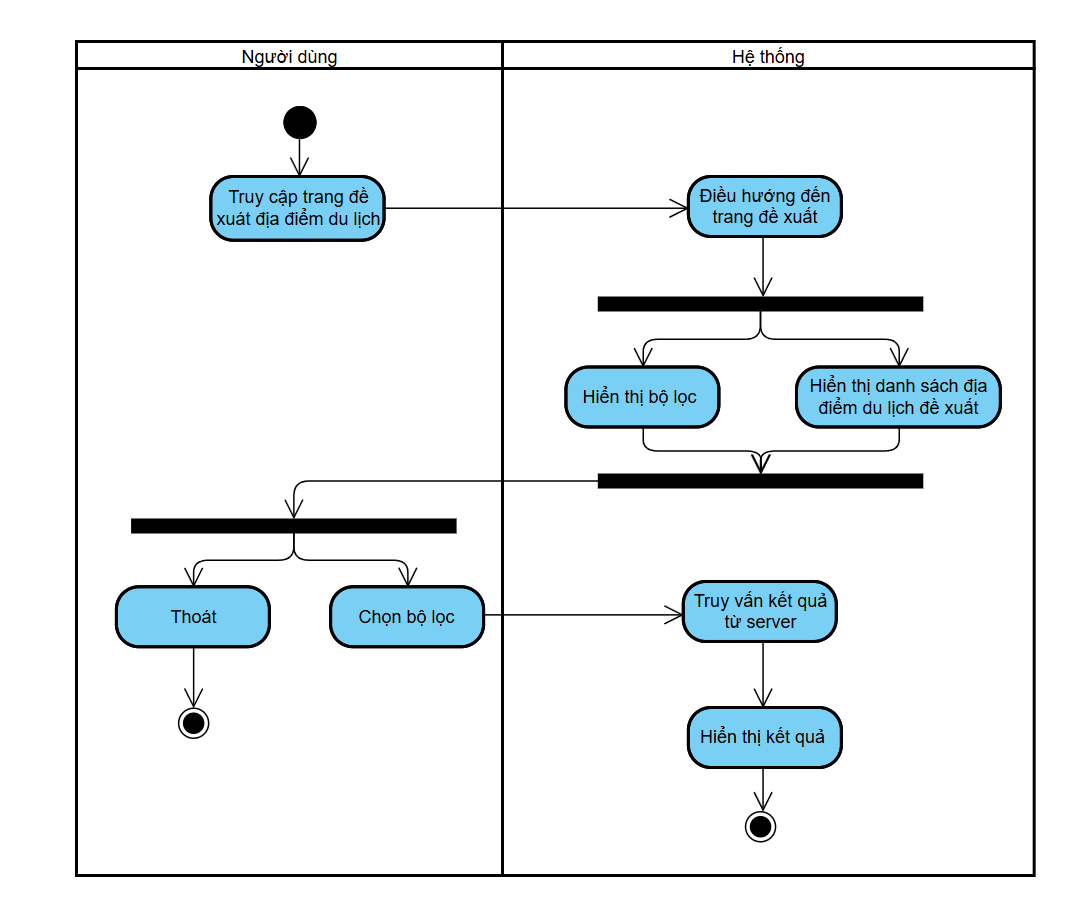
\includegraphics[width=0.5\linewidth]{figures/c3/3-3-6-ad.png}
        &
        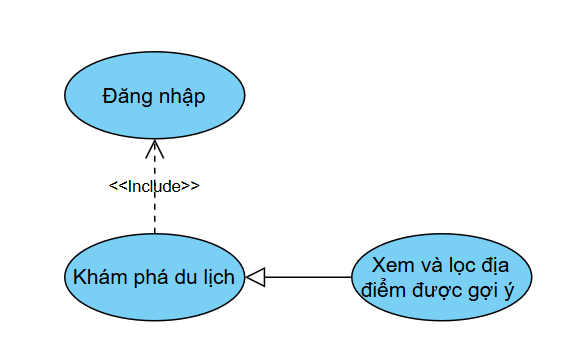
\includegraphics[width=0.45\linewidth]{figures/c3/3-3-6-rd.png} \\
        \hline
    \end{tabular}
\end{table}

\begin{figure}[H]
    \centering
    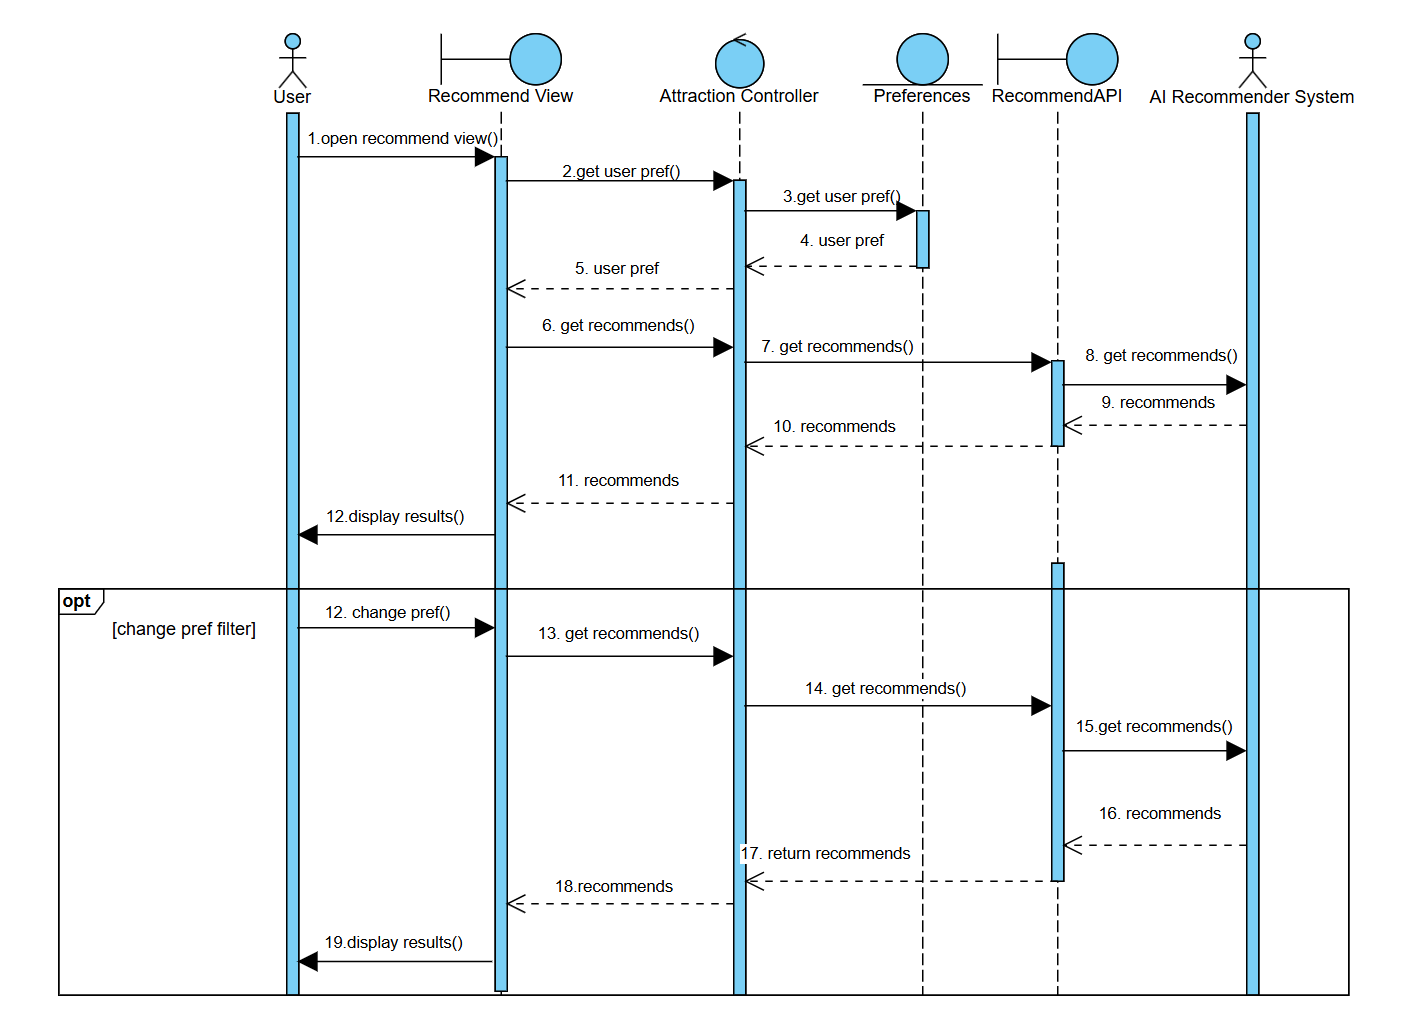
\includegraphics[width=1\textwidth]{figures/c3/3-3-6-sd.png} % Adjusted width slightly
    \caption{Biểu đồ tuần tự ca sử dụng xem danh sách địa điểm được gợi ý.}
    \label{fig:3-3-6-sequence-diagram}
\end{figure}